This calculator employs an event-based Monte Carlo simulation approach to
probabilistic risk assessment in order to estimate the loss distribution for
individual assets and aggregated loss distribution for a spatially distributed
portfolio of assets within a specified time period. The calculator requires
the definition of an \gls{exposuremodel}, a \gls{vulnerabilitymodel} for each loss type
of interest with \glspl{vulnerabilityfunction} for each taxonomy represented in the
\gls{exposuremodel}, and a set of ground motion fields representative of the
seismicity of the region over the specified time period. Loss curves and loss
maps can currently be calculated for five different loss types using this
calculator: structural losses, nonstructural losses, contents losses, downtime
losses, and occupant fatalities. The main results of this calculator are loss
exceedance curves for each asset, which describe the probability of exceedance
of different loss levels over the specified time period, and loss maps for the
region, which describe the loss values that have a given probability of
exceedance over the specified time period. Aggregate loss exceedance curves
can be also be produced using this calculator; these describe the probability
of exceedance of different loss levels for all assets in the portfolio. Finally,
event loss tables can be produced using this calculator; these tables describe
the total loss across the portfolio for each seismic event in the stochastic
event set.

This calculator relies on the probabilistic event-based hazard calculator,
which simulates the seismicity of the chosen time period $T$ by producing a
\textit{stochastic event set} (also known as a \textit{synthetic catalog}).
For each rupture generated by a source, the number of occurrences in the given
time span $T$ is simulated by sampling the corresponding probability
distribution as given by $P_{rup}(k | T)$. A stochastic event set is therefore
a \textit{sample} of the full population of ruptures as defined by a seismic
source model. Each rupture is present zero, one or more times, depending on
its probability. Symbolically, we can define a stochastic event set ($SES$)
as:
\begin{align}
SES(T) = \left\{k \times rup,\;k\sim P_{rup}(k | T)\;\;\forall\;rup\;in\;Src\;\forall\;Src\;in\;SSM\right\}
\end{align}
where $k$, the number of occurrences, is a random sample of $P_{rup}(k | T)$,
and $k \times rup$ means that rupture $rup$ is repeated $k$ times in the
stochastic event set.

For each rupture or event in the stochastic event sets, a spatially correlated
ground motion field (GMF) realisation is generated, taking into consideration
both the inter-event variability of ground motions, and the intra-event
residuals obtained from a spatial correlation model for ground motion
residuals. The use of logic trees allows for the consideration of uncertainty
in the choice of a seismic source model, and in the choice of GMPE models for the
different tectonic regions.

For each GMF realization, a loss ratio is sampled for every asset in the
\gls{exposuremodel} using the provided probabilistic vulnerability model, taking
into consideration the correlation model for vulnerability of different assets
of a given taxonomy. Finally loss exceedance curves are computed for both
ground-up losses and insured losses.

The required input files required for running a probabilistic stochastic
event-based risk calculation and the resulting output files are depicted in
Figure~\ref{fig:io-structure-event-based-risk}

\begin{figure}[ht]
\centering
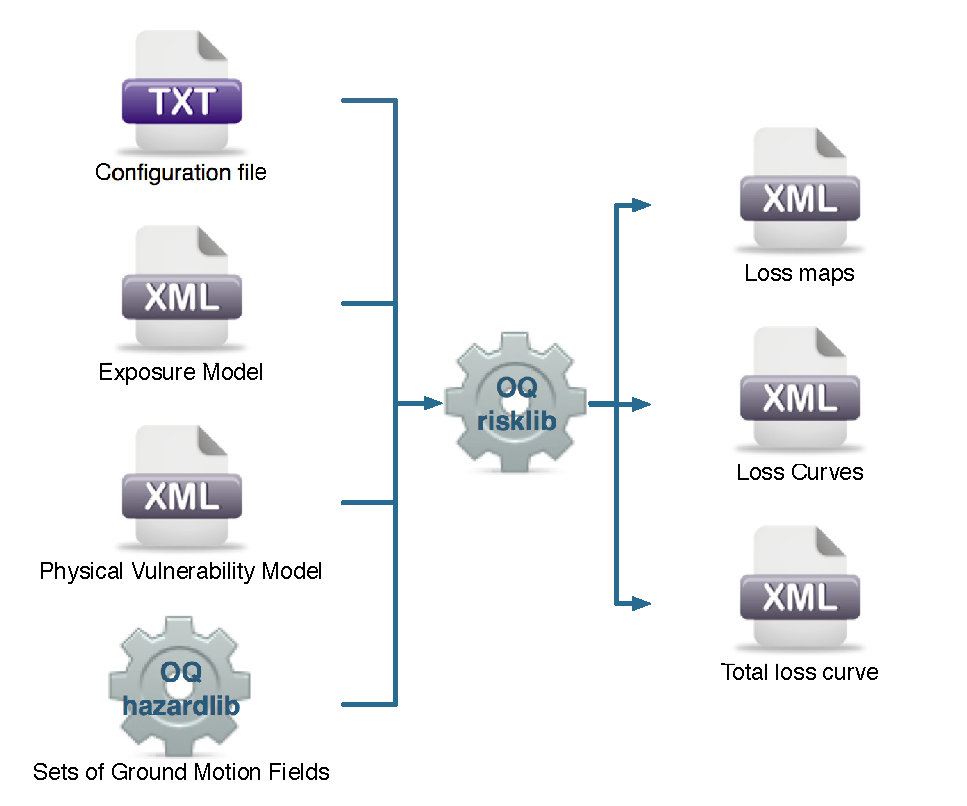
\includegraphics[width=9cm,height=7cm]{figures/risk/io-structure-event-based-risk.pdf}
\caption{Probabilistic Event-based Risk Calculator input/output structure.}
\label{fig:io-structure-event-based-risk}
\end{figure}
